\documentclass[UTF8,12pt,a4paper]{ctexart}
\usepackage{amsmath,amssymb,booktabs,array,geometry,graphicx,float,placeins}
\usepackage[hidelinks]{hyperref}
\geometry{left=2.5cm,right=2.5cm,top=2.5cm,bottom=2.5cm}
\setlength{\parindent}{2em}\linespread{1.25}
\newcommand{\keywords}[1]{\par\vspace{.5em}\noindent\textbf{关键词：}#1}
\title{基于离散频谱与可识别性约束的外延层厚度分析}\author{}\date{}
\begin{document}\pagenumbering{arabic}\maketitle\vspace{-2.5em}
\begin{abstract}
针对红外反射谱中折射率未知、波数非严格等距、异常测量与多光束机制难区分的问题，本文以一次反射、透射产生的两束干涉为基线，以等距波数上的$n$点 Hann 离散快速傅里叶变换为主模型。因缺少与样品、波段匹配的折射率和独立厚度真值，全文只报告光学量$q$及条件厚度$d(n)=q/\sqrt{n^2-\sin^2\theta_0}$，不把它们解释为唯一真实厚度。

问题一由 Snell 定律与往返相位推得相邻同类条纹的条件厚度关系，并完成量纲和法向退化核验。问题二在预先固定的W1（600--1600）、W2（1600--2800）、W3（2800--3800 cm$^{-1}$）中处理碳化硅双角数据，主模型$q$依次约为10.0009、20.8335、20.0018 $\mu$m；15$^\circ$数据在有依据掩码下仅W1变为10.0002 $\mu$m。双角、掩码结果接近而跨窗差异明显，故只能支持内部一致性。

问题三从界面反射、相干、衰减与仪器可分辨性推导多光束必要条件。硅数据三窗$q$约为15.0014、12.5001、10.0009 $\mu$m。预注册多光束双门未触发，机制证据不足、厚度影响未估计，故不执行修正。验证含432次合成和72个观测组合：F在相对误差不超过2.0的宽松阈值下144/144通过，但中位误差0.020883、最大1.000180（约100.018\%）；B通过率45.8333\%，P有36/144次失败；FFT压力变体使$q$最大变化18.75\%。附件2的262个超100\%点及四文件首零值均如实保留。
\keywords{红外干涉；外延层厚度；离散快速傅里叶变换；光学厚度；多光束干涉}
\end{abstract}\clearpage

\section{问题重述与分析}
题目给出同一碳化硅晶圆和同一硅晶圆在10$^\circ$、15$^\circ$入射下的反射谱，要求先建立一次反射、透射的两束模型，再计算碳化硅厚度并评价可靠性，最后讨论多光束必要条件、判断硅数据并给出相应结果。题目未提供匹配的折射率曲线、仪器相干长度或独立厚度真值，因而首要难点不是强行得到单一数值，而是区分可识别的光学量与依赖折射率的几何厚度。

本文采用“B基线---F主模型---P补充诊断---M条件准入”的冻结路线。B用局部极值间距，直观但易受峰值配对和稀疏条纹影响；F利用整个窗口的离散频率峰；P不覆盖F；只有机制证据和稳定显著的厚度影响同时成立时才准许M。三个固定窗口、两角度及raw/reasoned口径全部报告，不按结果选窗。

表\ref{tab:contract}给出三问的输出契约及结论边界。

\begin{table}[H]\centering\small
\caption{逐问输出契约}\label{tab:contract}
\begin{tabular}{p{1.2cm}p{4.2cm}p{4.5cm}p{4.2cm}}\toprule
问题&输出&粒度&边界\\\midrule
一&相位式、$q$、$d(n)$&波数、角度、折射率符号&不代入无来源折射率\\
二&SiC逐窗条件结果&3窗$\times$2角$\times$2口径&内部一致性不等于准确\\
三&必要条件、三态判断、Si结果&同上并含M状态&证据不足不等于不存在\\\bottomrule
\end{tabular}\end{table}

后续公式统一使用表\ref{tab:symbols}中的核心符号；局部辅助量在相应公式旁定义。

\section{假设与符号}
在固定局部窗口内把$n\cos\theta_1$视为有效常量；空气折射率取1；外延层横向均匀、界面平行；窗口内吸收忽略或由低频基线吸收；双角观测共享物理厚度但先独立估计。跨窗漂移只用于限制外推，不允许事后改窗。

\begin{table}[H]\centering\small\caption{主要符号}\label{tab:symbols}
\begin{tabular}{lll}\toprule 符号&含义&单位/定义域\\\midrule
$\sigma$&波数&cm$^{-1}$\\ $\theta_0,\theta_1$&空气侧、层内角&rad\\
$n,\kappa$&线性折射率实部、消光系数&无量纲\\ $d$&几何厚度&$\mu$m，$d>0$\\
$q$&频谱识别的条件光学量&$\mu$m\\ $R$&反射率比例&无量纲\\\bottomrule
\end{tabular}\end{table}

\section{问题一：两束干涉模型}
由Snell定律，$\sin\theta_1=\sin\theta_0/n(\sigma)$。外延层往返相位为
\begin{equation}\phi=4\pi n(\sigma)d_{\rm cm}\cos\theta_1\,\sigma+\phi_r,\qquad d_{\rm cm}=10^{-4}d.\label{eq:phase}\end{equation}
两束近似下$R(\sigma)=a(\sigma)+b(\sigma)\cos\phi+\varepsilon$。若窗口内$n\cos\theta_1$及反射相位缓变，相邻同类极值满足$\Delta\phi\approx2\pi$，从而
\begin{equation}d=\frac{10^4}{2\Delta\sigma\sqrt{n^2-\sin^2\theta_0}},\quad
q=d\sqrt{n^2-\sin^2\theta_0},\quad d(n)=\frac{q}{\sqrt{n^2-\sin^2\theta_0}}.\label{eq:dn}\end{equation}
有效域为$n>\sin\theta_0$。式\eqref{eq:phase}中$d_{\rm cm}\sigma$无量纲；$\theta_0\to0$时退化为$d=10^4/(2n\Delta\sigma)$。该耦合说明没有匹配$n(\sigma)$便不存在唯一$d$。薄膜反射谱的FFT测厚也以此相位结构为基础\cite{Quinten2019FFTThickness}。

F先在每窗去除二次趋势，线性插值到$n$个等距波数点，乘$n$点Hann窗并作不零填充的rFFT；屏蔽直流和第1箱，从第2箱起选离散峰。峰频率$f_k$给出
\begin{equation}\widehat q_F=5000f_k,\qquad \delta q_F=5000/(\sigma_{\max}-\sigma_{\min}).\label{eq:fft}\end{equation}
$\delta q_F$是离散分辨率，不是置信区间。等距自变量、有限窗口、泄漏和色散均限制FFT解释\cite{Quinten2019FFTThickness}。

\begin{figure}[H]\centering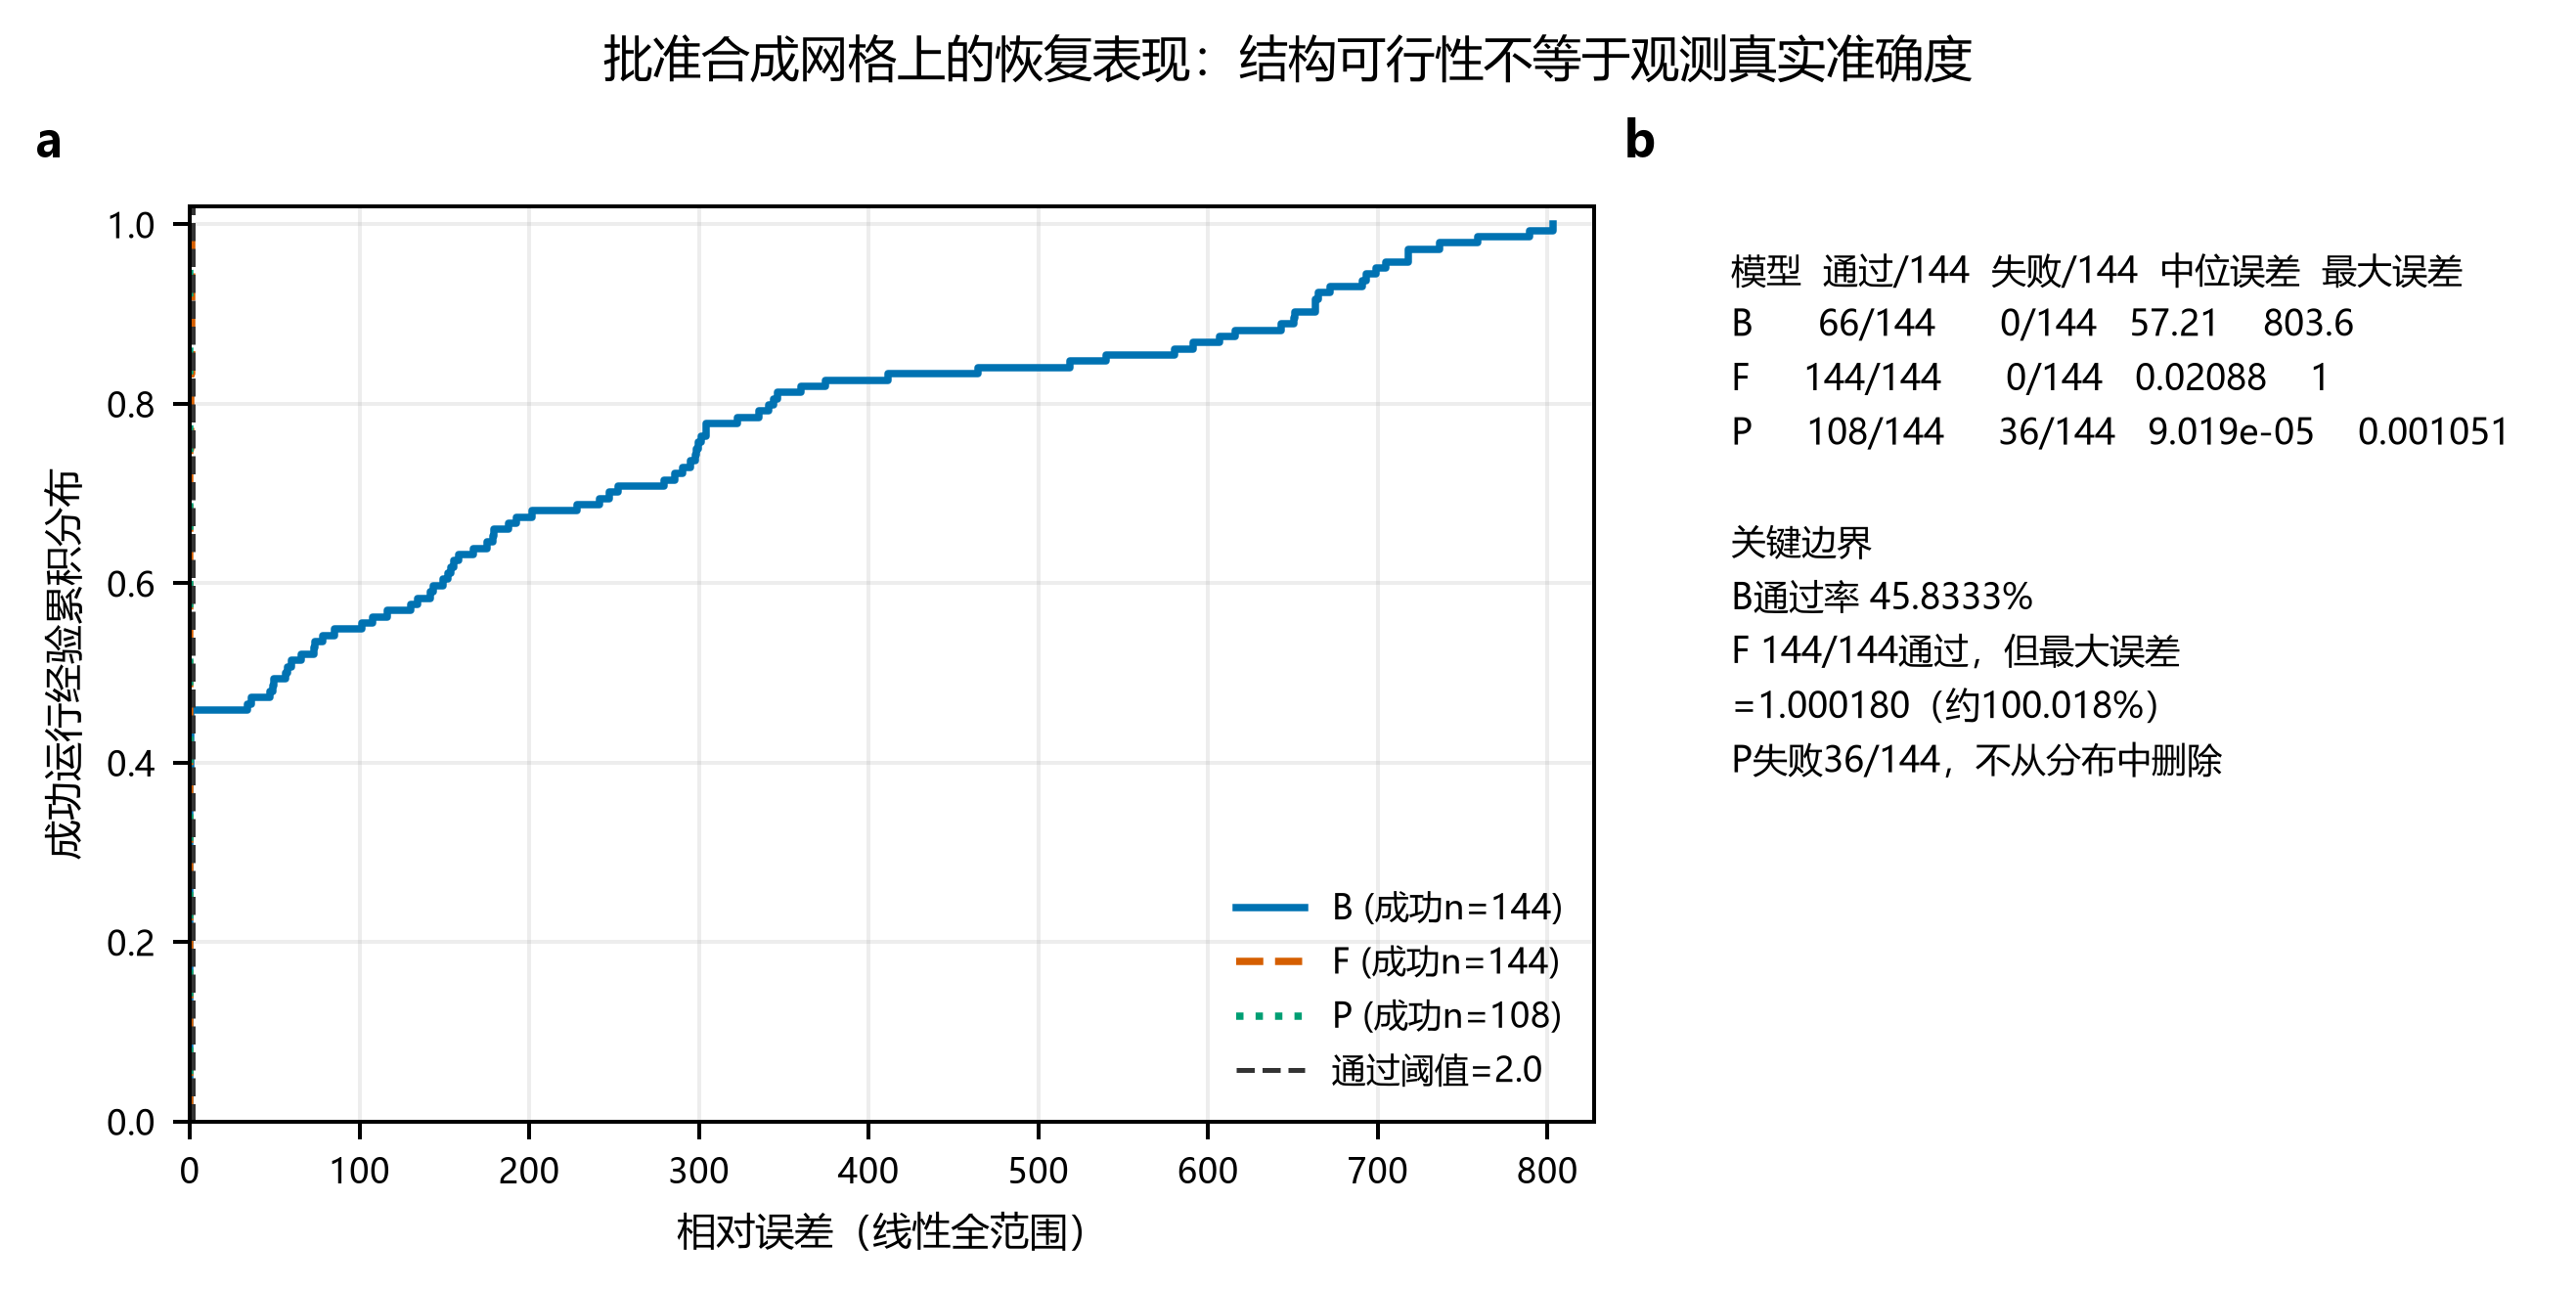
\includegraphics[width=.92\textwidth]{figs/FIG-SYNTH.png}
\caption{B、F、P的合成恢复；每模型144次，阈值为相对误差不超过2.0。}\label{fig:q1-synth}\end{figure}
图\ref{fig:q1-synth}中F为144/144通过，但中位相对误差0.020883、最大1.000180，故只支持批准合成模型下的结构可行性。B通过率45.8333\%；P有36次失败，只作补充诊断。

\clearpage
\section{问题二：碳化硅结果与可靠性}
四附件各7469点，波数严格递增但非精确等距。主分析保留原值；掩码仅作成对敏感性。附件2有262个$R>100\%$点，四表各有首零值，共266条排除记录，异常成因未知。

\begin{figure}[H]\centering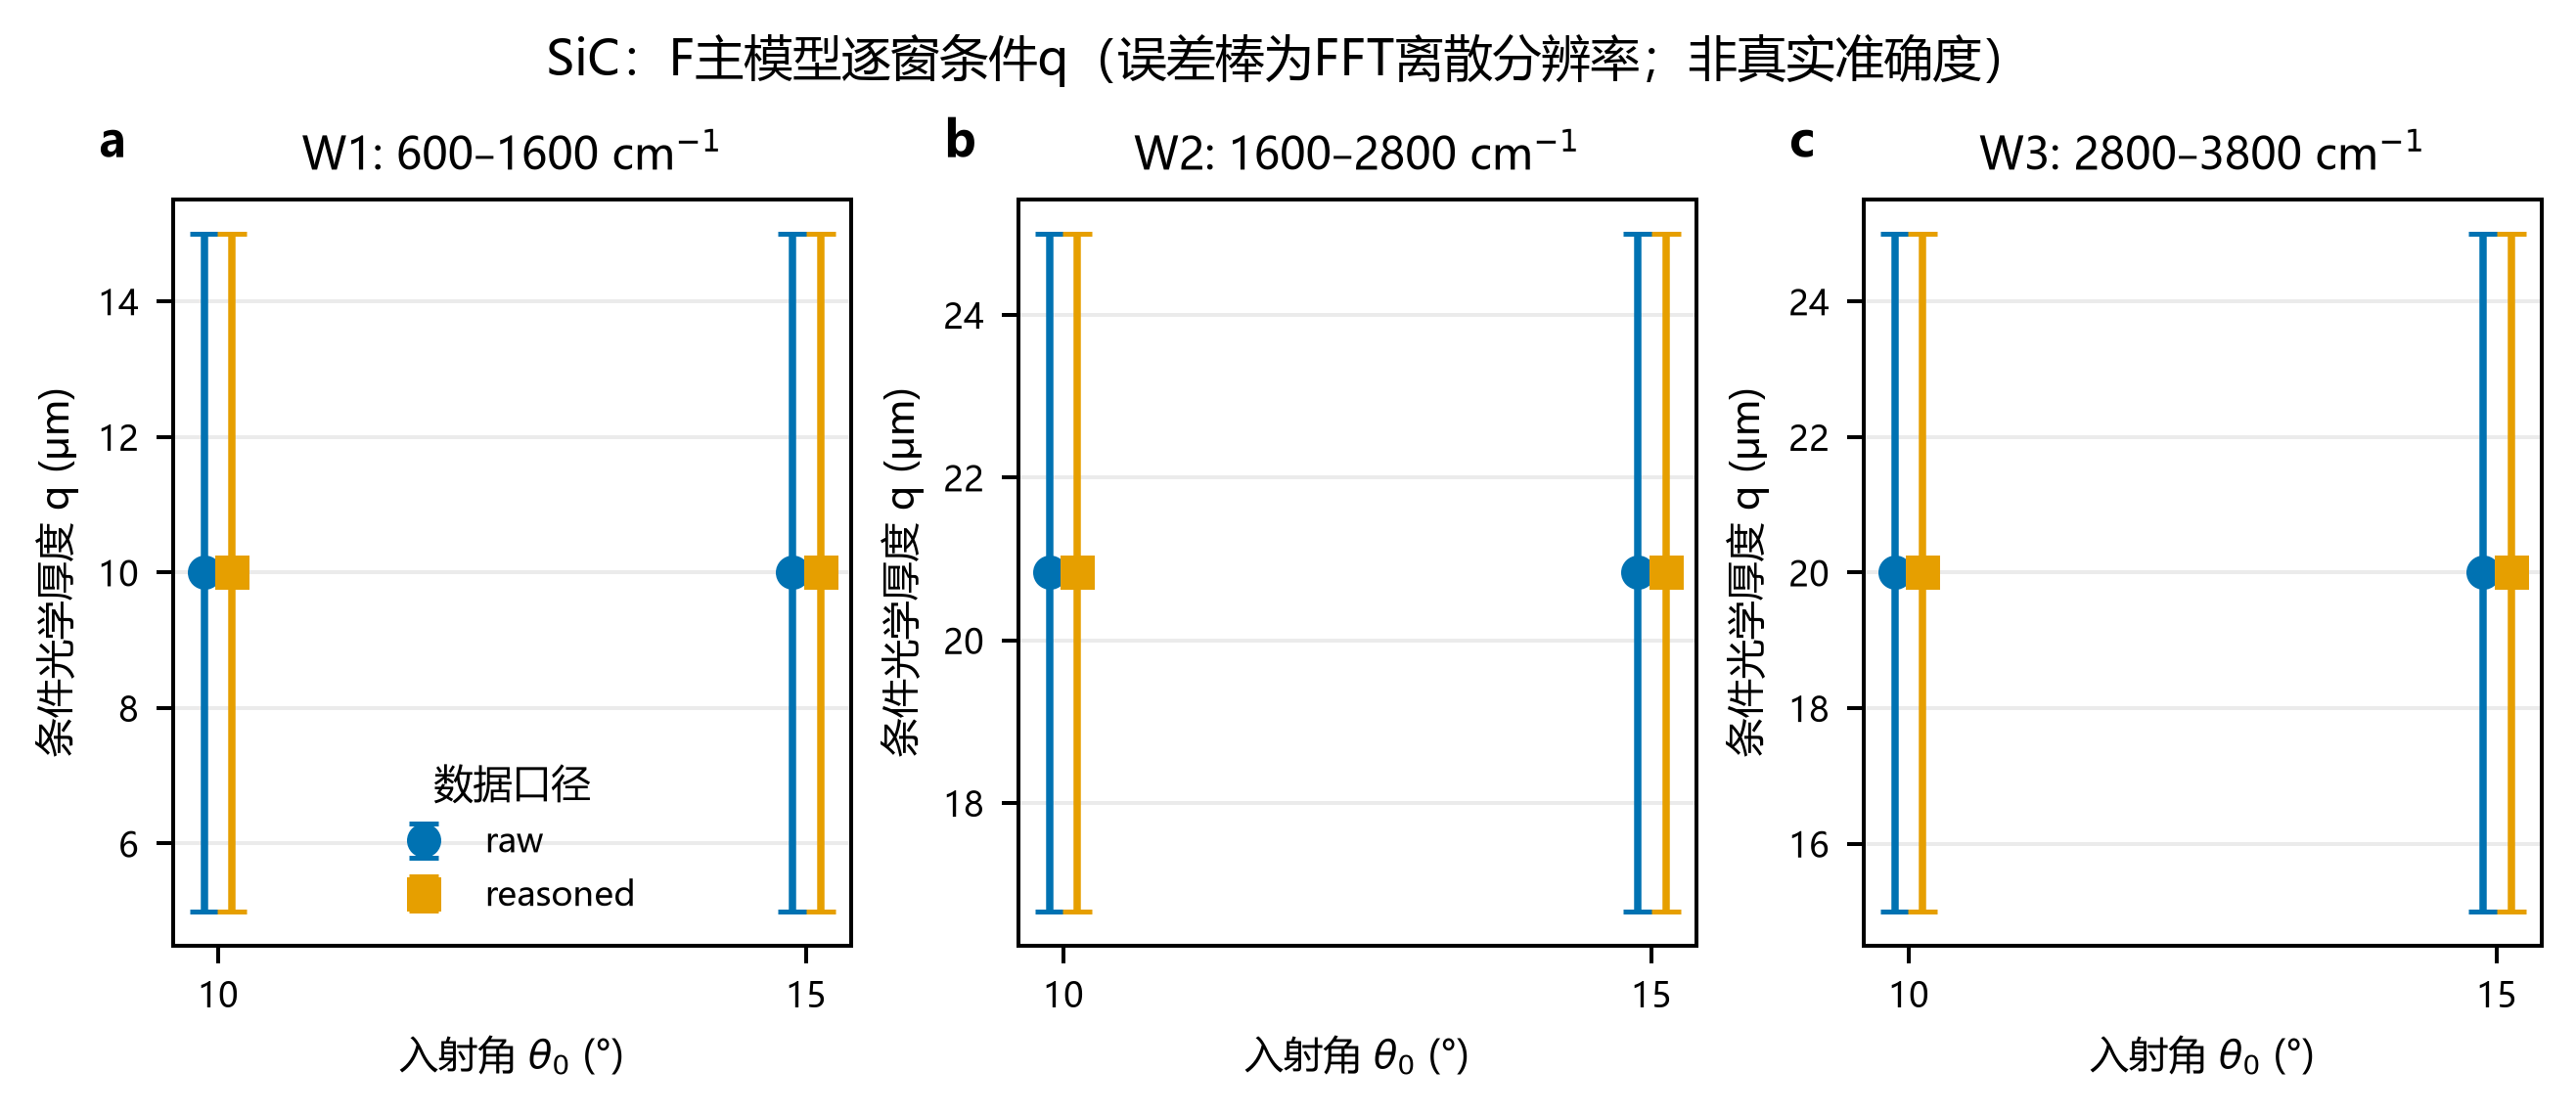
\includegraphics[width=.92\textwidth]{figs/FIG-Q2-F.png}
\caption{SiC三窗口、双角、双口径的F结果；误差棒为离散$q$分辨率。}\label{fig:q2-f}\end{figure}
图\ref{fig:q2-f}按冻结口径并列展示全部SiC窗口，不作跨窗平均。
\begin{table}[H]\centering\small\caption{SiC的F模型$q$（$\mu$m）}\label{tab:sic}
\begin{tabular}{ccccc}\toprule 角度&口径&W1&W2&W3\\\midrule
10$^\circ$&raw/reasoned&10.00090&20.83352&20.00180\\
15$^\circ$&raw&10.00090&20.83352&20.00180\\
15$^\circ$&reasoned&10.00020&20.83352&20.00180\\\bottomrule\end{tabular}\end{table}
任意经团队批准且满足有效域的$n$均可代入式\eqref{eq:dn}换算条件厚度；当前没有批准的$n$数值边界，故不列唯一厚度。仅15$^\circ$ W1受掩码影响，相对变化约$6.98\times10^{-5}$；同窗双角近乎一致。然而SiC跨窗相对范围约0.639，跨窗差异显著，不能用双角一致性替代真实准确度。

\begin{figure}[H]\centering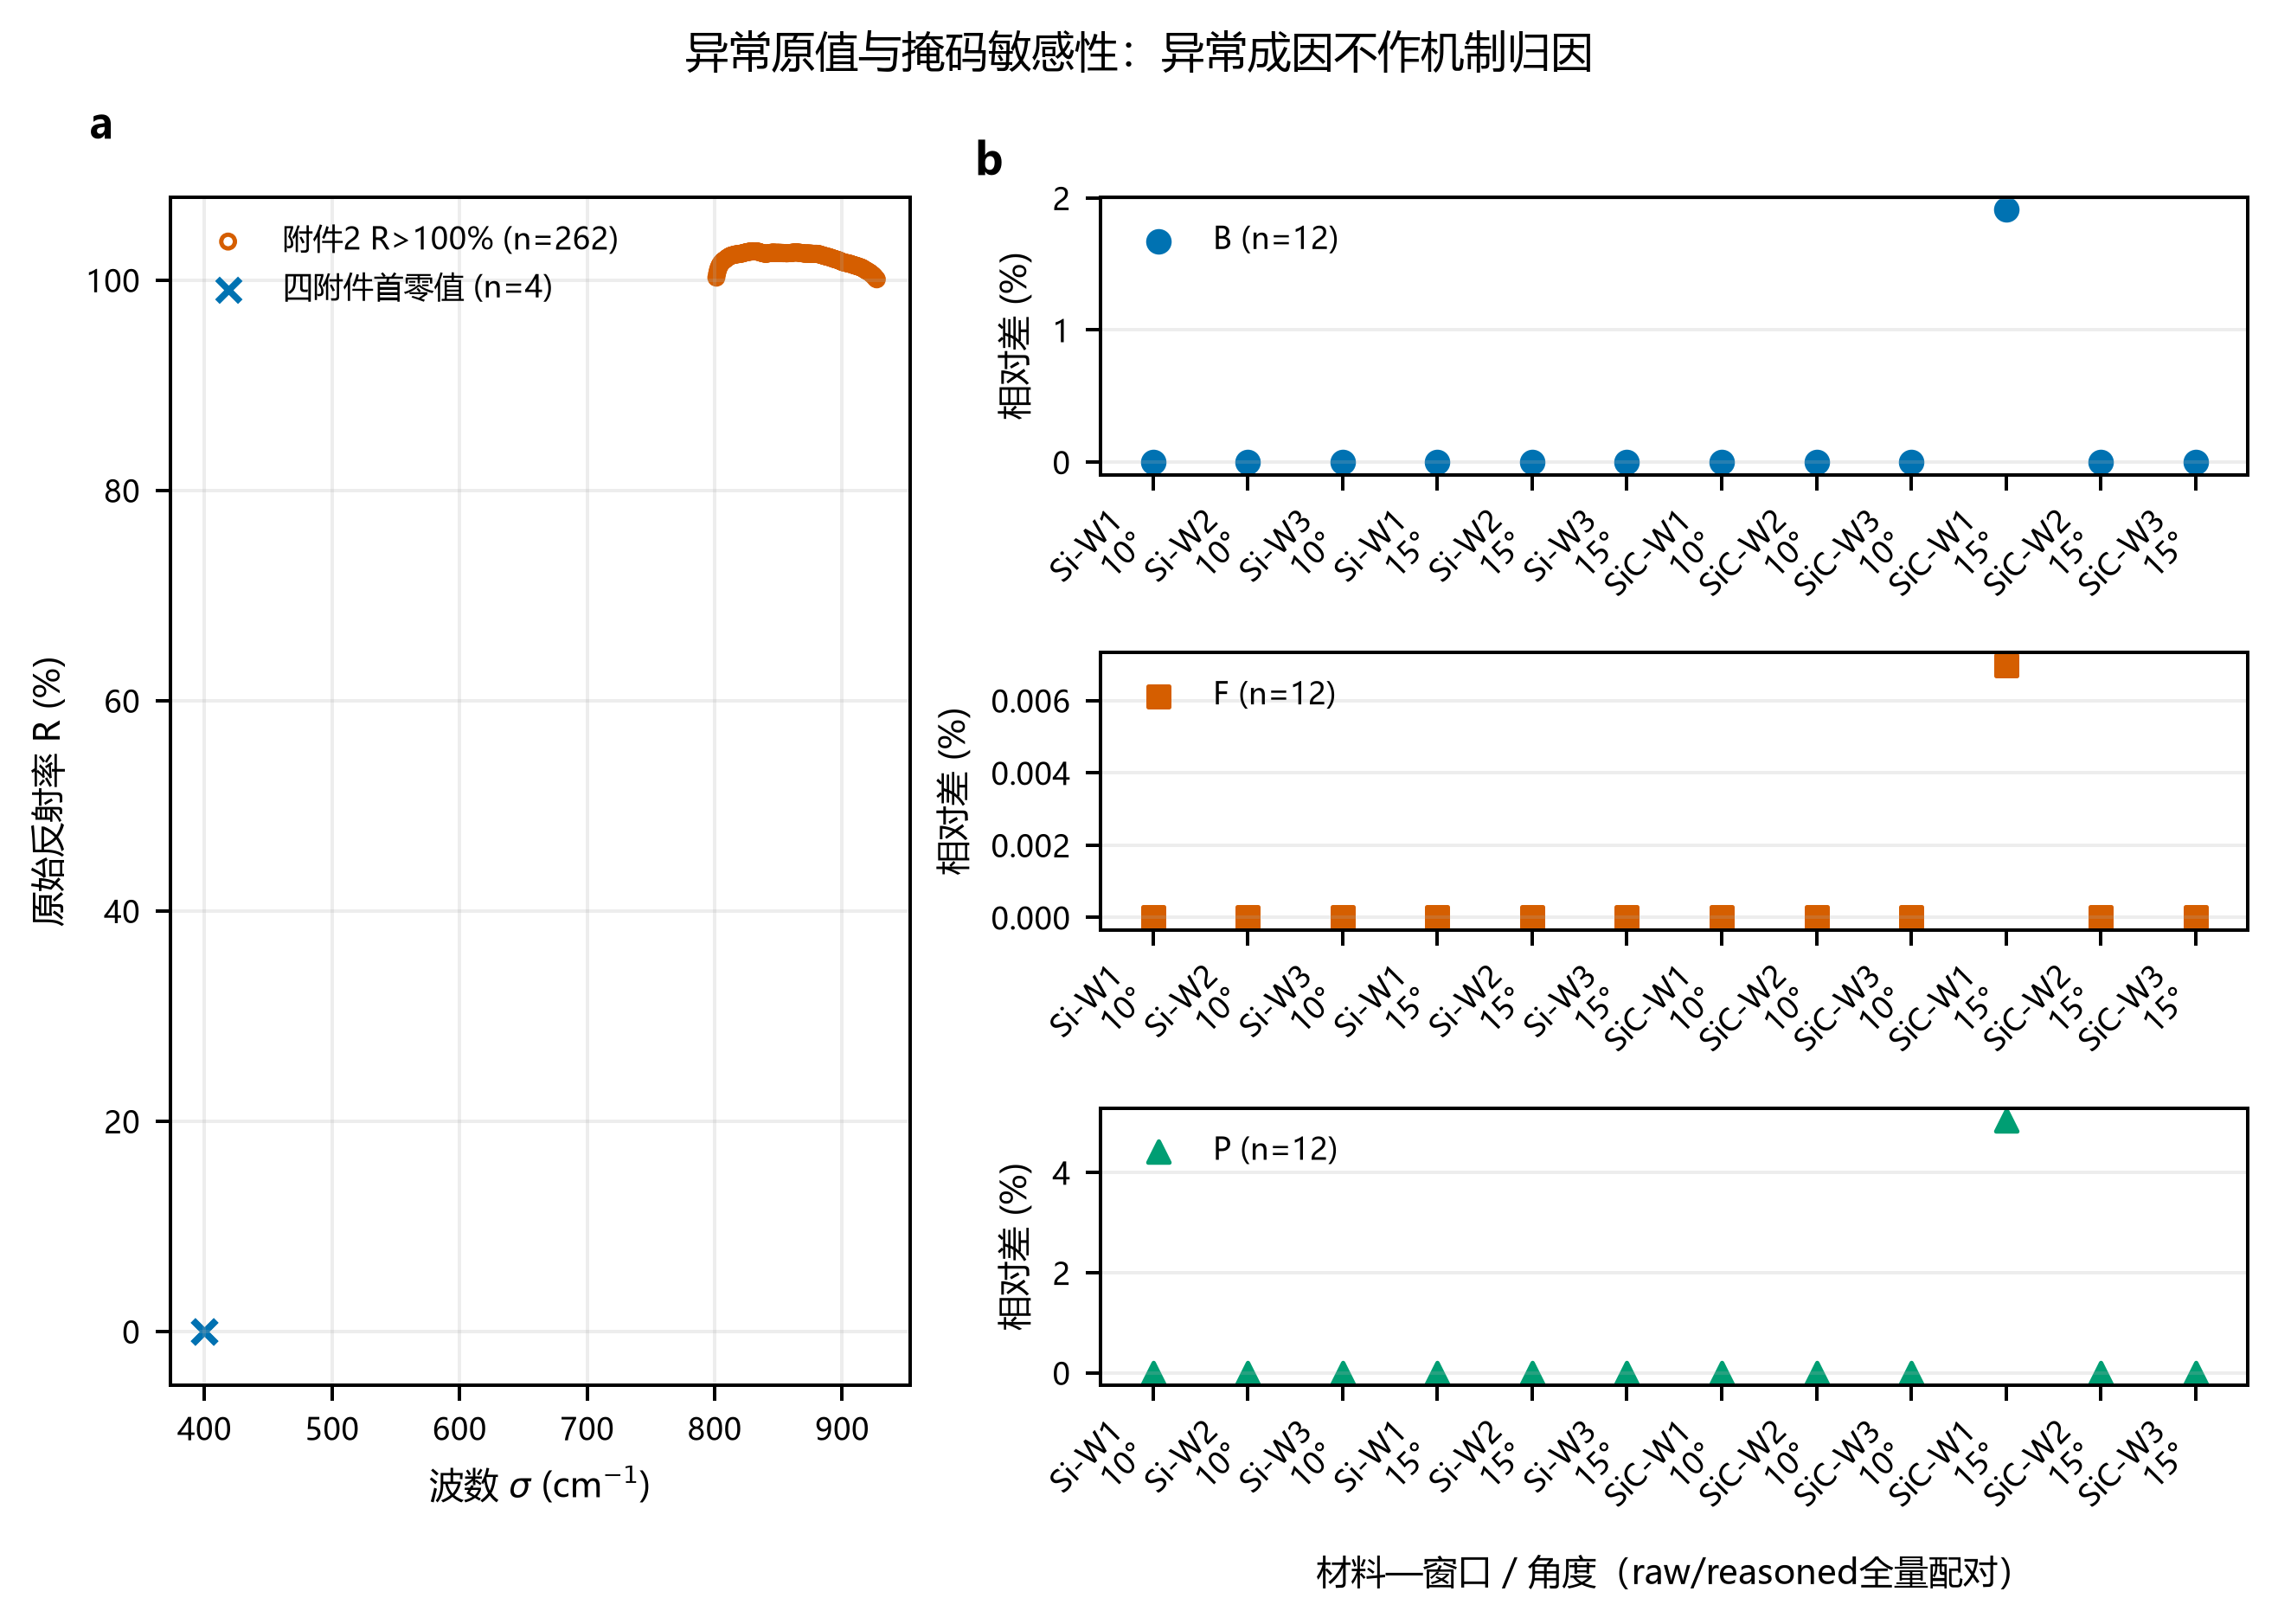
\includegraphics[width=.92\textwidth]{figs/FIG-MASK.png}
\caption{异常位置及raw/reasoned敏感性；异常不裁剪、不预归因为多光束。}\label{fig:q2-mask}\end{figure}
\begin{figure}[H]\centering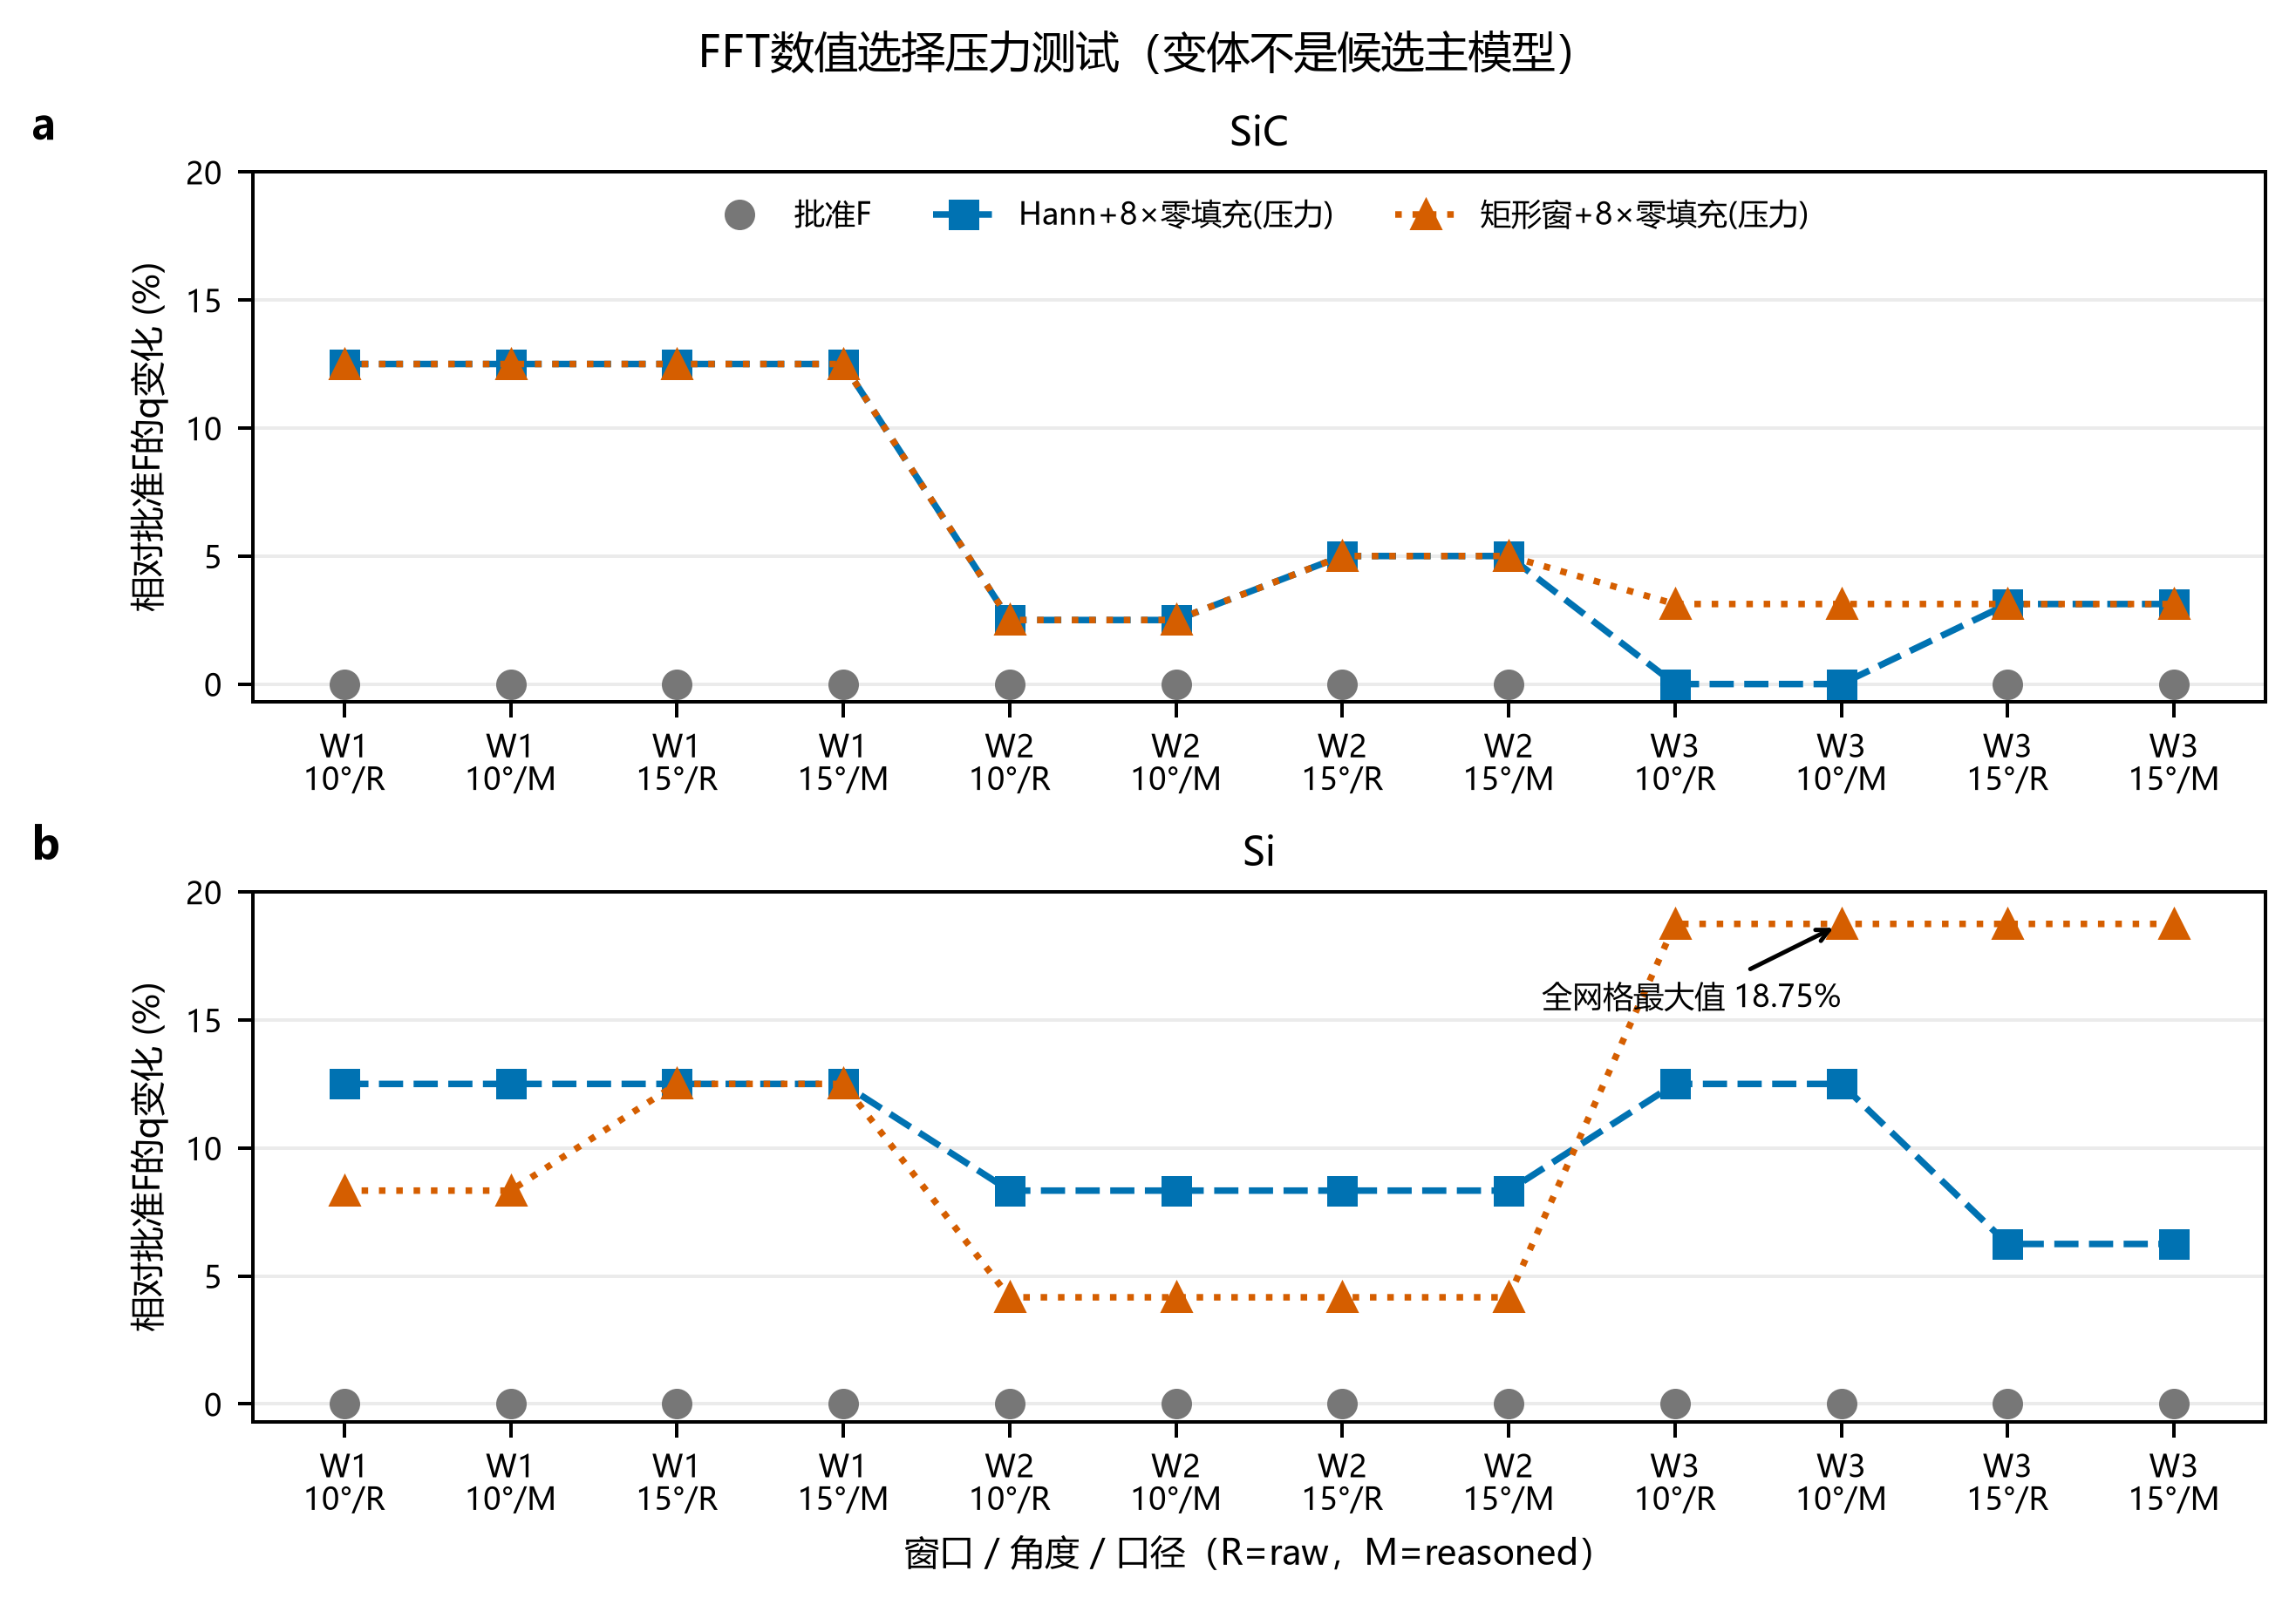
\includegraphics[width=.92\textwidth]{figs/FIG-ROBUST.png}
\caption{FFT压力测试；72个组合中$q$最大相对变化18.75\%。}\label{fig:q2-robust}\end{figure}
\clearpage
\begin{samepage}
图\ref{fig:q2-mask}定位异常并比较双口径，图\ref{fig:q2-robust}汇总冻结主模型与压力变体。Hann八倍零填充变体最大变化12.50\%，矩形窗八倍零填充最大变化18.75\%。这些变体仅揭示数值敏感性，不能覆盖冻结的$n$点Hann主结果。约5--6 $\mu$m的频率箱分辨率还表明，小数显示并非相同精度的物理测量。
\end{samepage}

\section{问题三：多光束条件与硅数据}
设界面复振幅反射系数为$r_{01},r_{12}$，单次往返传播因子
\begin{equation}g=r_{10}r_{12}\exp(2i\beta-2\alpha d/\cos\theta_1),\quad \beta=2\pi nd_{\rm cm}\sigma\cos\theta_1.\label{eq:g}\end{equation}
多次返回含$1+g+g^2+\cdots$。可观测多光束干涉至少要求：相关界面反射非零；光程差处于相干能力内；吸收、粗糙度、楔度和散射未完全抑制高阶返回；相位变化可由仪器分辨；各束偏振和空间重叠足够。复折射率和分层传播是处理该机制的一般框架\cite{Ballester2025ThinFilmFormulae}，吸收参数则依赖波长与载流子状态，不能脱离适用域迁移\cite{BakerFinch2014SiliconAbsorption}。

上述均为必要而非充分条件。$r_{12}\to0$、强衰减使$|g|\to0$、或失相干平均移除交叉项时，高阶项分别退化。退化检查通过不证明实测中存在多光束。

\begin{figure}[H]\centering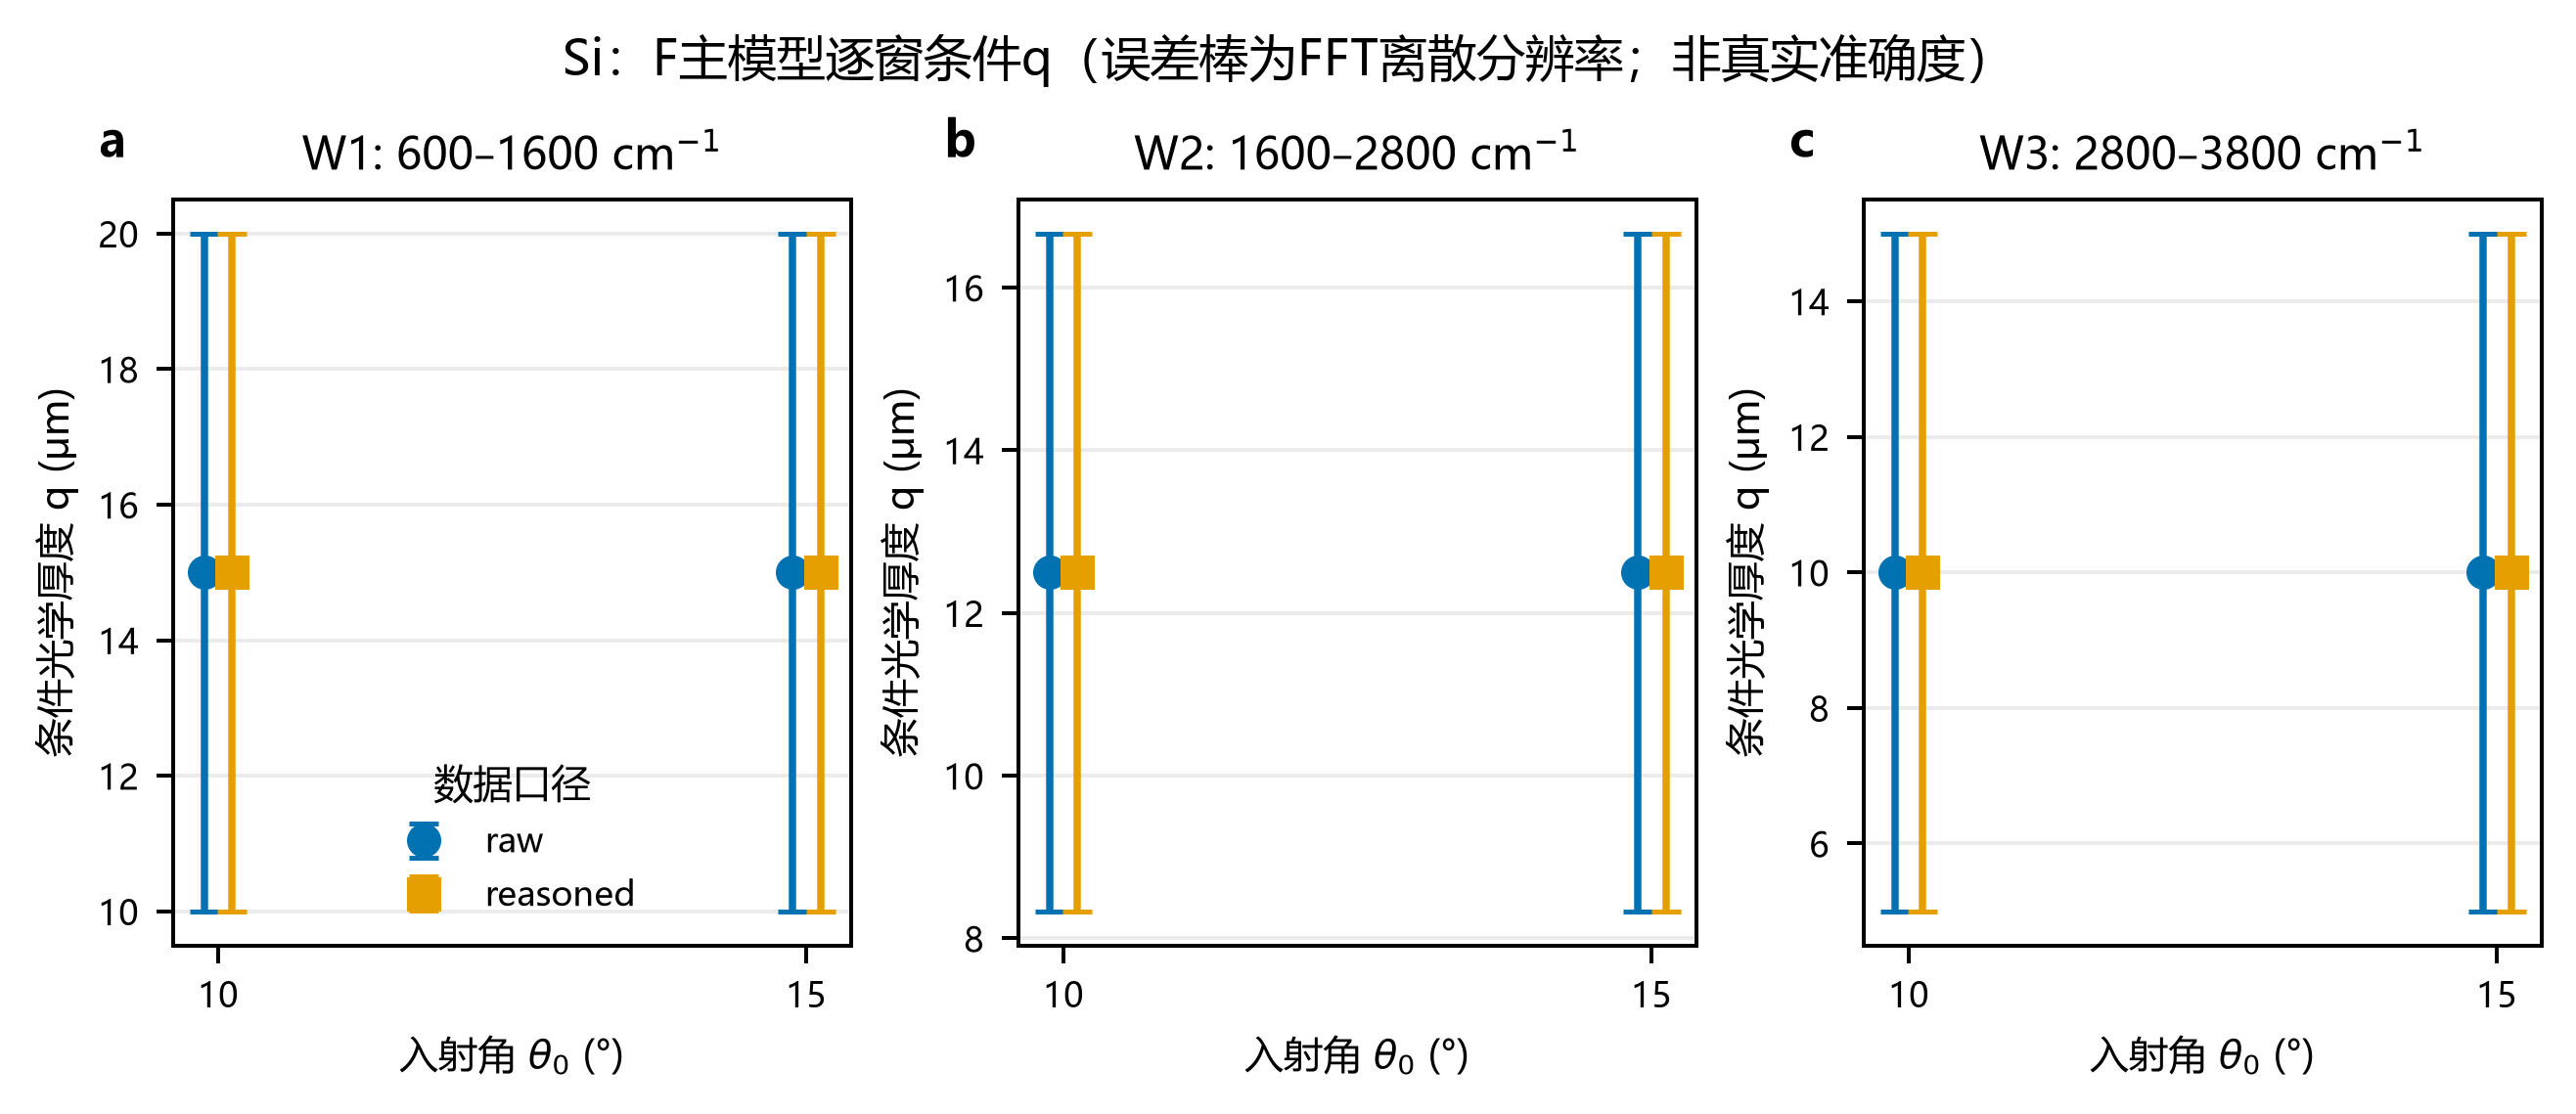
\includegraphics[width=.92\textwidth]{figs/FIG-Q3-F.png}
\caption{Si三窗口、双角、双口径的条件$q$；不跨窗平均。}\label{fig:q3-f}\end{figure}
图\ref{fig:q3-f}显示Si数据在同窗内双角、双口径一致，但窗口之间发生系统变化。
\begin{table}[H]\centering\small\caption{Si的F模型$q$（$\mu$m）}\label{tab:si}
\begin{tabular}{ccccc}\toprule 角度&口径&W1&W2&W3\\\midrule
10$^\circ$&raw/reasoned&15.00135&12.50011&10.00090\\
15$^\circ$&raw/reasoned&15.00135&12.50011&10.00090\\\bottomrule\end{tabular}\end{table}
每窗双角与双口径相同，而跨窗相对范围约0.400。色散、吸收、频率分辨率、楔度及仪器基线均是替代解释，现有证据不能唯一归因多光束。SiC材料存在多型与制备迁移风险，文献中的非线性折射率也不能代替本题线性折射率\cite{Ou2023SiCPhotonics}。

\begin{table}[H]\centering\small\caption{多光束M的准入与退化状态}\label{tab:m}
\begin{tabular}{p{3.6cm}p{4.5cm}p{5.8cm}}\toprule 项目&状态&解释\\\midrule
准入&{\scriptsize\ttfamily GATE\_\allowbreak NOT\_\allowbreak TRIGGERED}&双门未触发，M关闭\\
机制证据&{\scriptsize\ttfamily INSUFFICIENT\_\allowbreak EVIDENCE}&证据不足不等于不存在\\
厚度影响&{\scriptsize\ttfamily NOT\_\allowbreak ESTIMATED}&不生成修正结果\\
反射趋零/强衰减/失相干&三项退化检查通过&高阶或相位项按对应极限消失\\\bottomrule\end{tabular}\end{table}
机制证据与稳定显著的厚度影响必须同时成立才准入M。当前第一门不足、第二门未估计，因此Si和SiC均不执行修正，也不虚构修正前后结果。
表\ref{tab:m}据此保留三态判断及三项退化检查，避免把“证据不足”误写为“不存在”。

\section{验证、评价与边界}
最终代码完整运行约5.97 s，生成432条合成、72条观测和84条验证记录。量纲和退化检查验证公式--程序一致性；合成恢复验证批准结构下的算法恢复；双角、跨窗、掩码及压力测试只验证内部稳定性。它们均不等价于外部真值验证。

模型优点在于物理相位与代码对应、固定窗口全报、失败与异常不隐藏，并以$q$和$d(n)$区分可识别量。局限包括匹配$n,\kappa$、独立真值、相干长度、角度误差、粗糙度与楔度均缺失；局部常量假设不能跨窗外推；离散FFT分辨率较粗。若获得适用域明确的$n,\kappa$，可先冻结来源再计算$d(n)$区间；若获得独立厚度真值，方可评价真实误差。只有双角、跨窗结构残差与厚度影响同时越过预设门槛，才应重开M。

\section*{AI工具使用声明}
本研究在题目结构化、候选模型整理、代码实现与调试、全量计算、证据映射、正式图表、LaTeX写作和自动校验中使用了Codex任务环境中的配置模型。H1、H2、H3的路线和主张由队长明确决定。现有记录证明了程序复现、哈希校验、独立任务复核和团队闸门选择，但不能据此声称全文已由队员逐字人工核验。工具、用途、影响范围、采纳和核验状态见支撑材料《AI工具使用详情.pdf》；最终人工审查和提交责任由参赛队承担。

\bibliographystyle{plain}\bibliography{references}
\appendix
\section{支撑材料清单与运行入口}
支撑材料含\texttt{code/}中的完整可运行代码，\texttt{data/}中的四份原始附件，\texttt{results/}中的全部结果与中间表，\texttt{logs/}中的复现清单、运行和独立复核记录，以及AI工具使用详情PDF。运行入口为：
\begin{verbatim}
python code/run_compute.py --project-root <恢复后的项目根目录>
\end{verbatim}
随机种子20260907；记录环境为Python 3.13.14、NumPy 2.5.2、Matplotlib 3.11.1。表\ref{tab:sic}、表\ref{tab:si}对应\texttt{results/observed\_all\_models.csv}；合成、压力、异常和M状态分别定位到\texttt{synthetic\_recovery.csv}、\texttt{fft\_pressure\_test.csv}、\texttt{mask\_exclusions.csv}和\texttt{M\_diagnostic.json}。
\end{document}
